\documentclass[12pt, a4paper]{article}
\usepackage[utf8]{inputenc}
\usepackage{graphicx}
\graphicspath{{./Figures/}}

\title{Milestone 1}
\author{Jack Byrnes, Raymond Ly}
\date{\today}
\pagenumbering{arabic}

\begin{document}
\maketitle
\tableofcontents

\section{UI and UX design}


\section{Database design}
It was necessary to design a database to allow our website to provide the information the user wants. A user must be able to make relational data queries such as 'show me the homeless ratio in LGA's that have a median weekly income lower than \$500'. We could have all of the information for the LGA's in the one table, with every attribute of that LGA in it's own column (eg. '2016\_homeless\_f\_0\_9' amount of female homeless people who are aged 0-9 in that LGA in 2016). With the current data we have, we would need 45 columns with that database design. \\

A table with 45 columns is manageable and if we did not want this project to be scalable, this design would be fine. We want the database to grow as more research is conducted however, and we would be starting to add columns to our database if all the information was in one table. This would require the database to make a copy of the table with the new columns, transfer all of the previous entries and delete the original. The amount of columns in the table would also become more and more unmanageable as more research data becomes available. If we split the data up into multiple tables we avoid this issue and any new data is added as new data entries (rows) without having to do a complete restructure.

To decide how many entities (table) we needed and which attributes (columns) each entity should have, we analysed the data that we have and made an entity diagram (see figure \ref{fig:erdiagram}). The database modelled in the diagram allows for entry of new data without making new attributes. 

\begin{figure}[h]
\centering
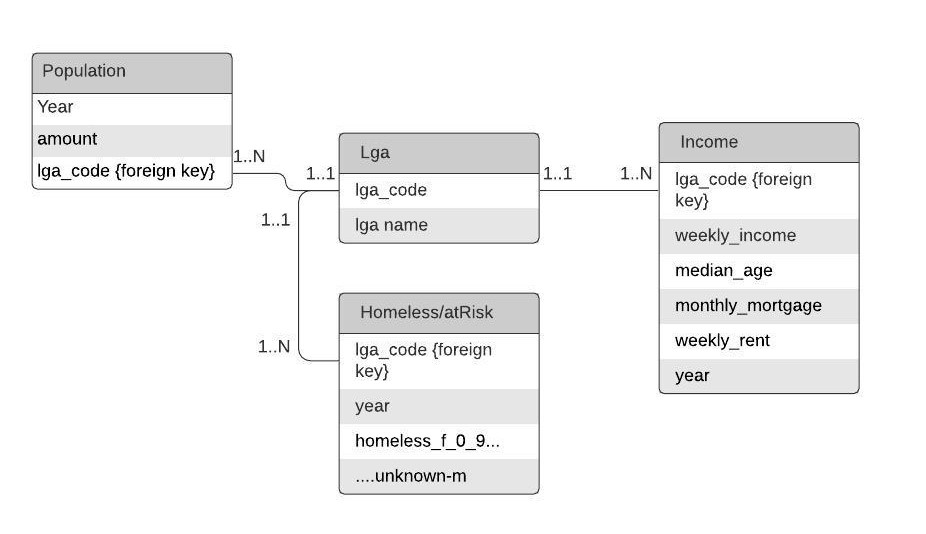
\includegraphics[scale=.8]{ERDiagram.jpg} 
\caption{Entity Relationship diagram of the diagram}
\label{fig:erdiagram}
\end{figure}

\textbf{Relational model}\\
A relational model can be extracted from this diagram:\\
Lga(\underline{lga\_code}, lga name)\\
Population(\underline{lga\_code*, year}, amount)\\
Income(\underline{lga\_code*, year}, weekly\_income, median\_age, monthly\_mortgage, weekly\_rent)\\
Homeless/AtRisk(\underline{lga\_code*, year}, **homeless\_f\_0\_9 ... unknown\_m )\\

\emph{**Note}: The Homeless/AtRisk entity has attributes between the ellipses. Each attribute is an integer amount of the people that meet the conditions stated. For example, the attribute 'homeless\_f\_0\_9' corresponds to people who are homeless, female and between the ages 0 and 9 inclusive. If this attribute were '7', the year attribute '2016' and the lga\_code was the code corresponding to Sunbury, it would mean there were 7 homeless female people aged 0-9 in 2016.\\

The database modelled in figure \ref{fig:erdiagram} enable the website to deliver any information that the user needs. As an example, lets look at how the database would work for a query. To illustrate it's capability we will choose a complex query:\\

\textbf{Query:} What is the ratio of homeless people against the total population in LGA's where the median weekly income is under \$500. We will assume the user wants the most recent data available and only use data from 2018
These are the steps that are needed in order to answer this query with the data that we have:
\begin{enumerate}
\item Find all of the LGA's that had a median weekly income under \$500 in 2018.
\item Calculate the total number of people in these LGA's who were homeless in 2018.
\item Find the total 2018 population of these LGA's.
\item Divide the result of step 2. by the result of step 3.
\end{enumerate}
In order to answer this query, our database would complete these steps:
\begin{enumerate}
\item Find all of the weekly\_income entries in the Income table that are less than 500 along with the corresponding LGA codes.
\item Find and sum the amounts of all homeless that correspond to these LGA codes in the Homeless/AtRisk table. (all of the attributes that begin with 'homeless' for each LGA.
\item Find and sum the amounts that corresponds to these codes and the year '2018' in the Population table.
\item Divide the result in step 2. by the result in step 3.
\end{enumerate} 

\textbf{Building the database:} \\
To build the database, we imported four csv files. Two files resembled two of the tables that we would need in the database: Population and Income. Another two files contained the information that we needed for our Homeless/AtRisk table. All of these files also contained the information needed to create the LGA table: LGA codes with corresponding LGA names. To build our database, we executed the following steps in Sqlite Studio:

\begin{enumerate}
\item Create a database and import all four csv files as tables using the GUI in Sqlite Studio. Resulting in tables: HRA2016, HRA2018, Population and Income.
\item Combine the 2016 and 2018 data on homeless people and people who are at risk of being homeless by executing: \\
\hspace*{10mm}%
INSERT INTO [HRA2018]\\
\hspace*{10mm}%
SELECT * FROM [HRA2016];\\
Then renaming HRA2018 to Homeless/AtRisk using the GUI.
\item Creating an LGA table and inserting the LGA code and name columns from the Income table (either Income or Population would have worked here):\\
\hspace*{10mm}%
CREATE TABLE [LGA](\\
\hspace*{10mm}%
lga\_code INT PRIMARY KEY NOT NULL,\\
\hspace*{10mm}%
lga\_name TEXT NOT NULL);\\
\hspace*{10mm}%
INSERT INTO [LGA]\\
\hspace*{10mm}%
SELECT lga\_code, lga\_name FROM Population;
\item Remove the column containing the LGA names from all tables excluding [LGA]. This can be done in a couple of ways, we chose to use the GUI.
\end{enumerate}

\end{document}
